%%%%%%%%%%%%%%%%%%%%%%%%%%%%%%%%%%%%%%%%%%%%%%%%%%%%%%%%%%%%%%%%%%%%%%
% Problem statement
\begin{statement}[
  problempoints=110,
  timelimit=1 second,
  memorylimit=512 MiB,
]{Klasika}

%\setlength\intextsep{-0.1cm}
%\begin{wrapfigure}[9]{r}{0.17\textwidth}
%\centering
%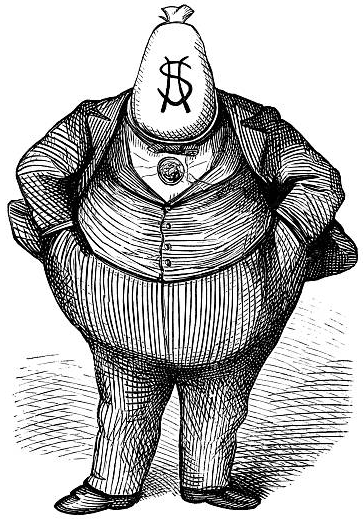
\includegraphics[width=0.17\textwidth]{img/holding.png}
%\end{wrapfigure}

In the beginning there was a node denoted as $1$ and it represented the root
of a tree. Your task is to support $Q$ queries of the form:

\begin{itemize}
  \item \texttt{Add x y} -- Adds a new node to the tree as a child of node $x$.
        The newly added node and node $x$ are connected with an edge of weight
        $y$. The newly added node is denoted by a number equal to the number
        of nodes that the tree consists of after its addition.
  \item \texttt{Query a b} -- Finds the longest path in a tree which starts in
        node $a$ and ends in some node from the subtree of node $b$ (which itself
        is considered to be in its own subtree). The length of the path is defined
        as exclusive or (xor) of weights of all edges that the path consists of.
\end{itemize}

%%%%%%%%%%%%%%%%%%%%%%%%%%%%%%%%%%%%%%%%%%%%%%%%%%%%%%%%%%%%%%%%%%%%%%
% Input
\subsection*{Input}
The first line contains an integer $Q$ $(1 \le Q \le 200\ 000)$ from the task
description.

The $i$-th of the next $Q$ lines contains the $i$-th query whose format
corresponds to one of the queries from the task description. Values $x$, $a$ and
$b$ will refer to an existing node at that moment and value $y$ will not be
greater than $2^{30}$.

%%%%%%%%%%%%%%%%%%%%%%%%%%%%%%%%%%%%%%%%%%%%%%%%%%%%%%%%%%%%%%%%%%%%%%
% Output
\subsection*{Output}
You should output an answer to each query of type \texttt{Query}. Each
answer should be printed in a separate line in the order in which
corresponding queries appear in the input.

%%%%%%%%%%%%%%%%%%%%%%%%%%%%%%%%%%%%%%%%%%%%%%%%%%%%%%%%%%%%%%%%%%%%%%
% Scoring
 \subsection*{Scoring}
{\renewcommand{\arraystretch}{1.4}
  \setlength{\tabcolsep}{6pt}
  \begin{tabular}{ccl}
 Subtask & Score & Constraints \\ \midrule
  1 & 11 & $Q \le 200$ \\
  2 & 22 & $Q \le 2\ 000$ \\
  3 & 33 & In all queries of type \texttt{Query} it holds $b=1$ \\
  4 & 44 & No additional constraints.
\end{tabular}}

%%%%%%%%%%%%%%%%%%%%%%%%%%%%%%%%%%%%%%%%%%%%%%%%%%%%%%%%%%%%%%%%%%%%%%
% Examples
\subsection*{Examples}
\begin{tabularx}{\textwidth}{X'X'X}
\sampleinputs{test/klasika.dummy.in.1}{test/klasika.dummy.out.1} &
\sampleinputs{test/klasika.dummy.in.2}{test/klasika.dummy.out.2} &
\sampleinputs{test/klasika.dummy.in.3}{test/klasika.dummy.out.3}
\end{tabularx}

%%%%%%%%%%%%%%%%%%%%%%%%%%%%%%%%%%%%%%%%%%%%%%%%%%%%%%%%%%%%%%%%%%%%%%
% We're done
\end{statement}

%%% Local Variables:
%%% mode: latex
%%% mode: flyspell
%%% ispell-local-dictionary: "croatian"
%%% TeX-master: "../hio.tex"
%%% End:
